%!TEX root = lot2.tex

%--------------------------CARTES NEUTRE------------------------------------------------------------------------------------------------

\begin{tikzpicture} %Recto
	%Fond
    \node[anchor=south west,inner sep=0] (carte) at (0,0) {
\includegraphics[width=7.1 cm, height=9.6 cm]{fonds/noir.png}};
    \node[anchor=center] at (carte.center) {
\includegraphics[width=\cardwidth cm, height=\cardheight cm]{fonds/fond_plan.png}};
\end{tikzpicture}

\begin{tikzpicture} %Verso
	%Fond
    \node[anchor=south west,inner sep=0] (carte) at (0,0) {
\includegraphics[width=7.1 cm, height=9.6 cm]{fonds/noir.png}};
    \node[anchor=center] at (carte.center) {
\includegraphics[width=\cardwidth cm, height=\cardheight cm]{fonds/fond_plan.png}};
\end{tikzpicture}

%%%%%%%%%%%%%%%%%%%%%%%%%%%%%%%%%%%%%%%%%%NEVER MISS A DROP
\begin{tikzpicture} %Recto
	%Fond
    \node[anchor=south west,inner sep=0] (carte) at (0,0) {
\includegraphics[width=7.1 cm, height=9.6 cm]{fonds/noir.png}};
    \node[anchor=center] at (carte.center) {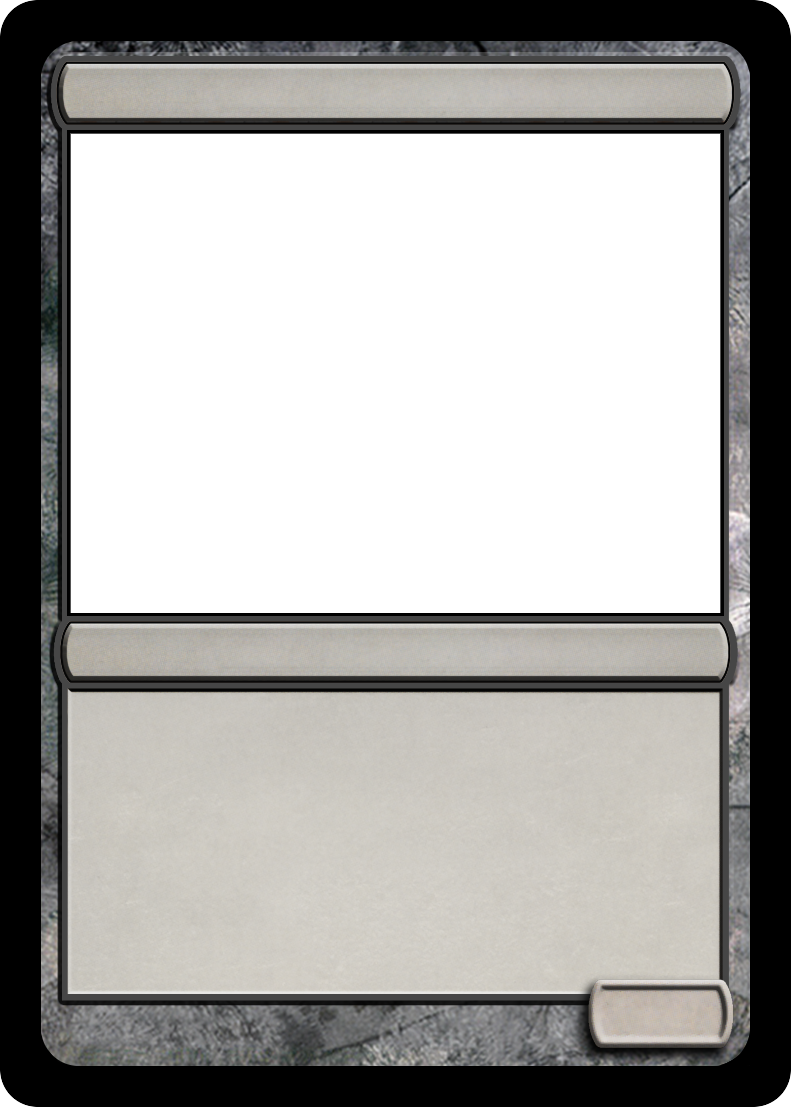
\includegraphics[width=\cardwidth cm, height=\cardheight cm]{fonds/fond_neutre.png}};

    %Titre
	\node[anchor=center] at (\titleX,\titleY) {\titlefont Never Miss A Drop !};

	%Image
	\node[anchor=center] at (\imageX,\imageY) {
\includegraphics[width=\imageWidth px, height=\imageHeight px]{images/never_miss.jpg}};
	\node[anchor=center] at (6.1,4.5) {
\includegraphics[width=12 px, height=6 px]{fonds2/legacy.jpg}};

	%Type
	\node[anchor=center] at (\typeX,\typeY) {\typefont Neutre};

	%Description
	\node[anchor=north west, text width=5.6cm] (description) at (\descriptionX,\descriptionY) {\descriptionfont\setsize{7} Grace au market piss, ne ratez plus une goutte ! Remplissez un verre d'eau à la hauteur de votre choix. Jusqu'à ce qu'un joueur déborde, chacun doit ajouter un NFT (faire couler de l'eau) dans le verre. Celui qui échoue doit piocher une carte, puis le tour se termine\par};

	%Punchline
	\node[anchor=north west, text width=5.6cm, below = 1pt of description] (punchline) {\punchlinefont\setsize{7}``Pour plus d'inclusivité, les toilettes d'entresol sont désormais agenrées.''\par};

	%Separateur !!!!!PAS TOUCHE!!!!!
	\fill[black,path fading=west] (description.south west) rectangle (punchline.north);
	\fill[black,path fading=east] (punchline.north) rectangle (description.south east);

	%Numéro !!!!!PAS TOUCHE!!!!!
	\node[anchor=center] at (\numberX,\numberY) {\numberfont \cardnumber};
\end{tikzpicture}\verso %Verso



%%%%%%%%%%%%%%%%%%%%%%%%%%%%%%%%%%%%%%%%%%HAN SOLO ROGERS
\begin{tikzpicture} %Recto
	%Fond
    \node[anchor=south west,inner sep=0] (carte) at (0,0) {
\includegraphics[width=7.1 cm, height=9.6 cm]{fonds/noir.png}};
    \node[anchor=center] at (carte.center) {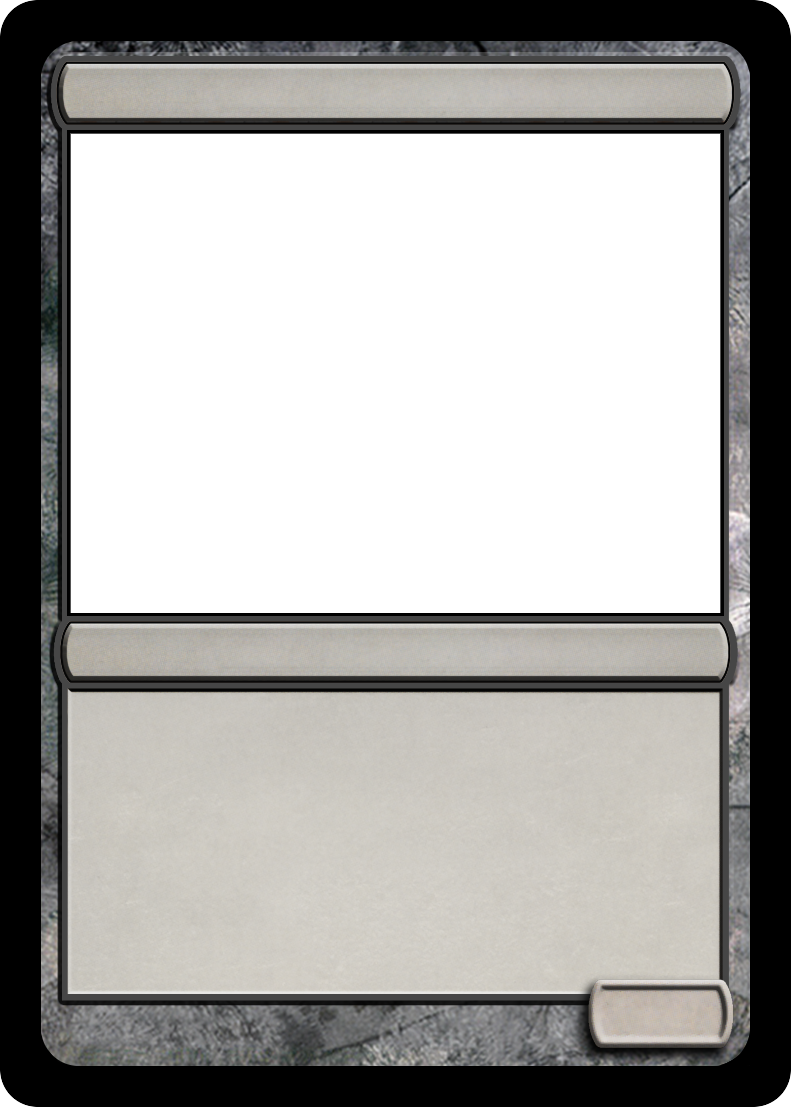
\includegraphics[width=\cardwidth cm, height=\cardheight cm]{fonds/fond_neutre.png}};

    %Titre
	\node[anchor=center] at (\titleX,\titleY) {\titlefont Han Solo Rogers};

	%Image
	\node[anchor=center] at (\imageX,\imageY) {
\includegraphics[width=\imageWidth px, height=\imageHeight px]{images/ian.jpg}};
	\node[anchor=center] at (6.1,4.5) {
\includegraphics[width=12 px, height=6 px]{fonds2/legacy.jpg}};

	%Type
	\node[anchor=center] at (\typeX,\typeY) {\typefont Neutre};

	%Description
	\node[anchor=north west, text width=5.6cm] (description) at (\descriptionX,\descriptionY) {\descriptionfont\setsize{7} Vous allez dégoter le futur artiste qui sera sponsorisé par le Market Pass ! Chaque joueur doit faire un dessin de singe. Vous choisissez le plus beau, l'auteur peut défausser une carte.\par};

	%Punchline
	\node[anchor=north west, text width=5.6cm, below = 1pt of description] (punchline) {\punchlinefont\setsize{7}``I have got a very good feeling about this.''\par};

	%Separateur !!!!!PAS TOUCHE!!!!!
	\fill[black,path fading=west] (description.south west) rectangle (punchline.north);
	\fill[black,path fading=east] (punchline.north) rectangle (description.south east);

	%Numéro !!!!!PAS TOUCHE!!!!!
	\node[anchor=center] at (\numberX,\numberY) {\numberfont \cardnumber};
\end{tikzpicture}\verso %Verso




%%%%%%%%%%%%%%%%%%%%%%%%%%%%%%%%%%%%%%%%%%SUICIDAL TENDENCIES
\begin{tikzpicture} %Recto
	%Fond
    \node[anchor=south west,inner sep=0] (carte) at (0,0) {
\includegraphics[width=7.1 cm, height=9.6 cm]{fonds/noir.png}};
    \node[anchor=center] at (carte.center) {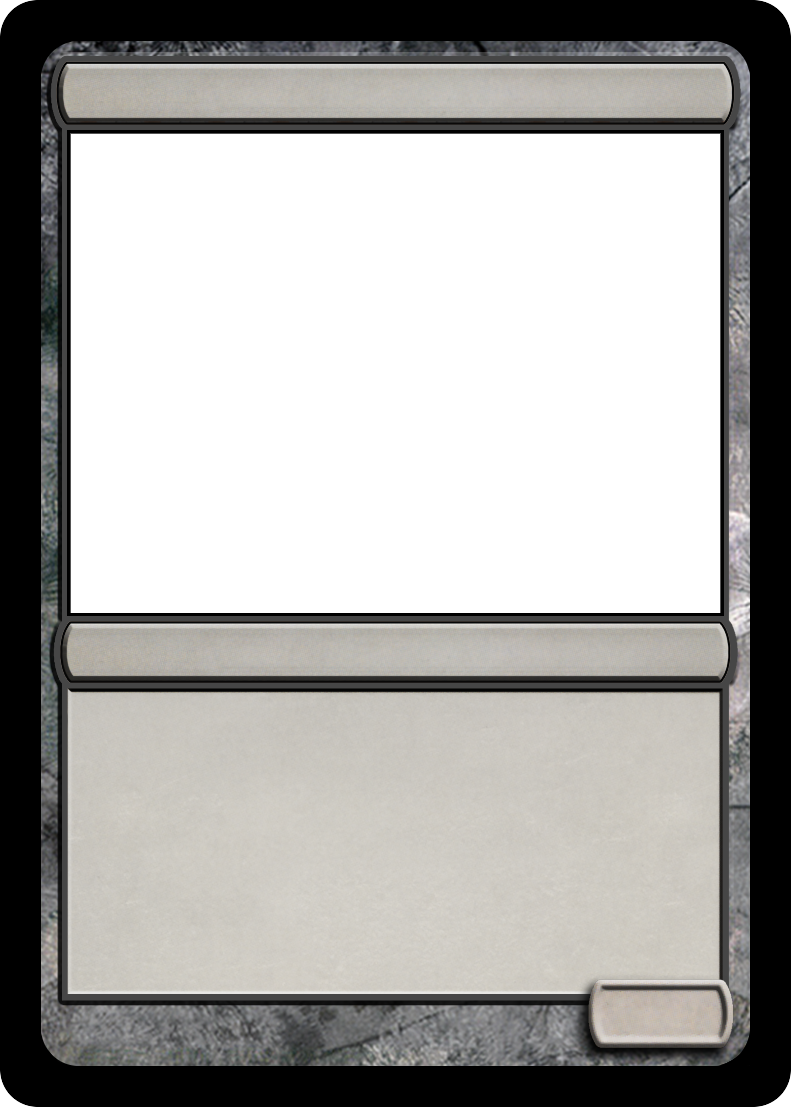
\includegraphics[width=\cardwidth cm, height=\cardheight cm]{fonds/fond_neutre.png}};

    %Titre
	\node[anchor=center] at (\titleX,\titleY) {\titlefont Suicidal Tendencies};

	%Image
	\node[anchor=center] at (\imageX,\imageY) {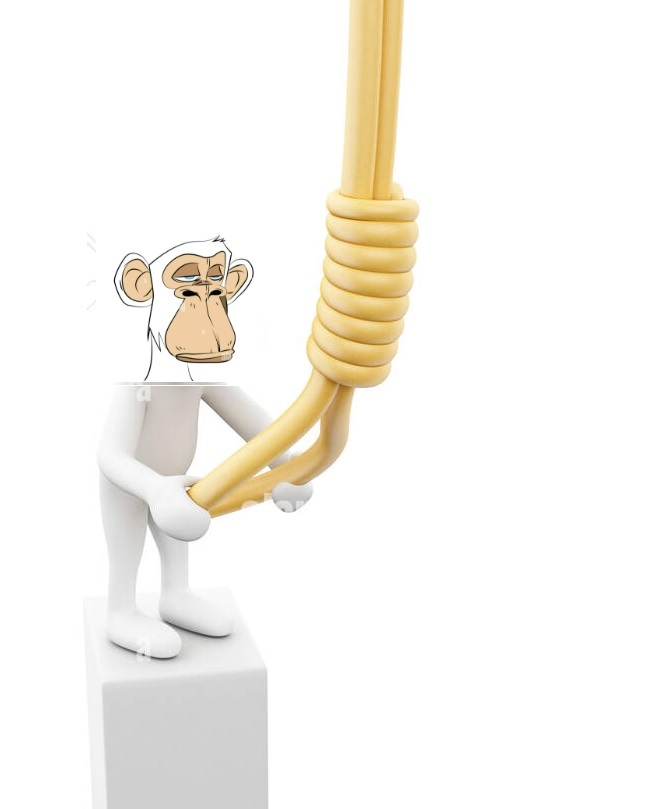
\includegraphics[width=\imageWidth px, height=\imageHeight px]{images/suicide.jpg}};
	\node[anchor=center] at (6.1,4.5) {
\includegraphics[width=12 px, height=6 px]{fonds2/legacy.jpg}};

	%Type
	\node[anchor=center] at (\typeX,\typeY) {\typefont Neutre};

	%Description
	\node[anchor=north west, text width=5.6cm] (description) at (\descriptionX,\descriptionY) {\descriptionfont\setsize{8} Cette carte peut être jouée si la carte {\emph Séminaire à Tenerife} est sur la table. Le joueur devant la carte décide subitement de confesser sa haine des NFT devant toute l'entreprise. Il crie Banzaï et pioche deux cartes.\par};

	%Punchline
	\node[anchor=north west, text width=5.6cm, below = 1pt of description] (punchline) {\punchlinefont\setsize{8}``Kevin Lombaire ne pouvait s'empècher de dire ce qu'il pensait. R.I.P. ''\par};

	%Separateur !!!!!PAS TOUCHE!!!!!
	\fill[black,path fading=west] (description.south west) rectangle (punchline.north);
	\fill[black,path fading=east] (punchline.north) rectangle (description.south east);

	%Numéro !!!!!PAS TOUCHE!!!!!
	\node[anchor=center] at (\numberX,\numberY) {\numberfont \cardnumber};
\end{tikzpicture}\verso %Verso



%%%%%%%%%%%%%%%%%%%%%%%%%%%%%%%%%%%%%%%%%%BUS
\begin{tikzpicture} %Recto
	%Fond
    \node[anchor=south west,inner sep=0] (carte) at (0,0) {
\includegraphics[width=7.1 cm, height=9.6 cm]{fonds/noir.png}};
    \node[anchor=center] at (carte.center) {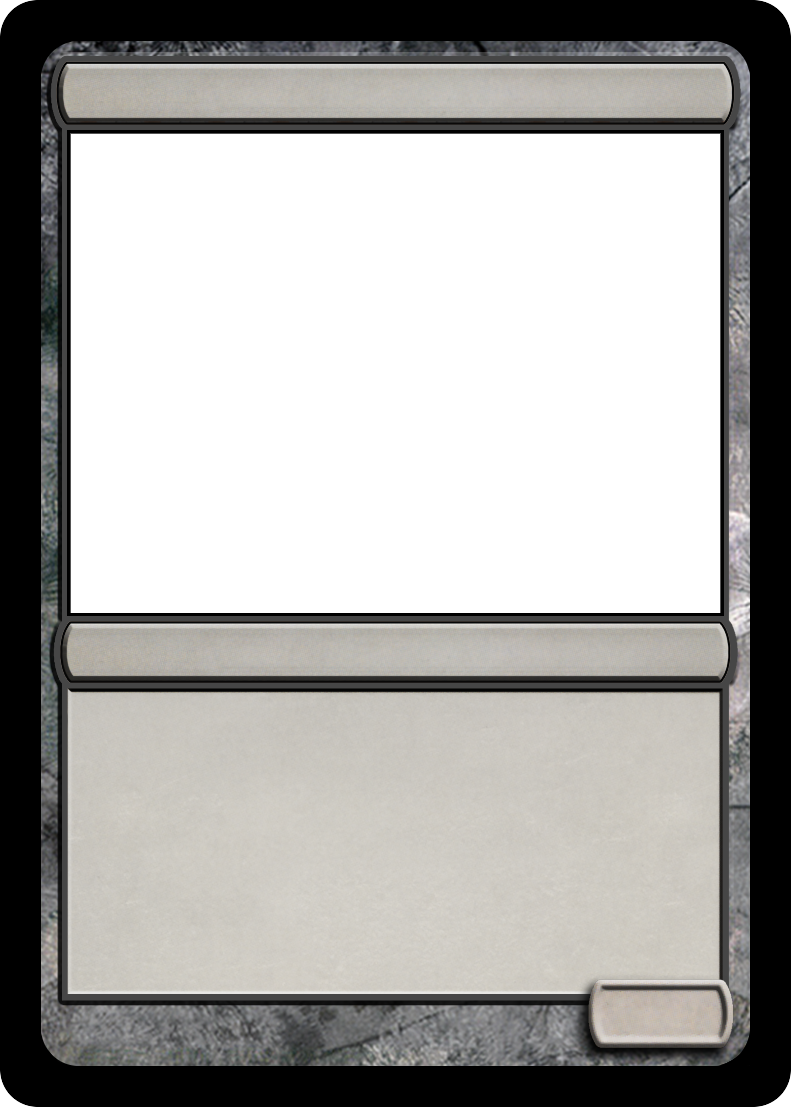
\includegraphics[width=\cardwidth cm, height=\cardheight cm]{fonds/fond_neutre.png}};

    %Titre
	\node[anchor=center] at (\titleX,\titleY) {\titlefont Bus pour Cosmos};

	%Image
	\node[anchor=center] at (\imageX,\imageY) {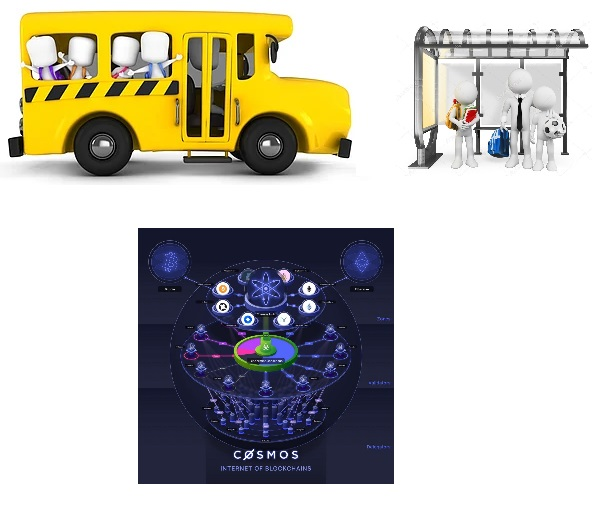
\includegraphics[width=\imageWidth px, height=\imageHeight px]{images/bus.jpg}};
	\node[anchor=center] at (6.1,4.5) {
\includegraphics[width=12 px, height=6 px]{fonds2/legacy.jpg}};

	%Type
	\node[anchor=center] at (\typeX,\typeY) {\typefont Neutre};

	%Description
	\node[anchor=north west, text width=5.6cm] (description) at (\descriptionX,\descriptionY) {\descriptionfont\setsize{8} Lorsque cette carte est jouée le stagiaire ne peut pas avoir de tour bonus car il préfère prendre le bus à la place. Ce dernier doit faire le tour de la pièce jusqu'à la fin du tour de jeu. Ben oui, c'est loin le cosmos !\par};

	%Punchline
	\node[anchor=north west, text width=5.6cm, below = 1pt of description] (punchline) {\punchlinefont\setsize{8}``Au moins Grand Corp Malade, lui il slamme. ''\par};

	%Separateur !!!!!PAS TOUCHE!!!!!
	\fill[black,path fading=west] (description.south west) rectangle (punchline.north);
	\fill[black,path fading=east] (punchline.north) rectangle (description.south east);

	%Numéro !!!!!PAS TOUCHE!!!!!
	\node[anchor=center] at (\numberX,\numberY) {\numberfont \cardnumber};
\end{tikzpicture}\verso %Verso



%%%%%%%%%%%%%%%%%%%%%%%%%%%%%%%%%%%%%%%%%%ENS 
\begin{tikzpicture} %Recto
	%Fond
    \node[anchor=south west,inner sep=0] (carte) at (0,0) {
\includegraphics[width=7.1 cm, height=9.6 cm]{fonds/noir.png}};
    \node[anchor=center] at (carte.center) {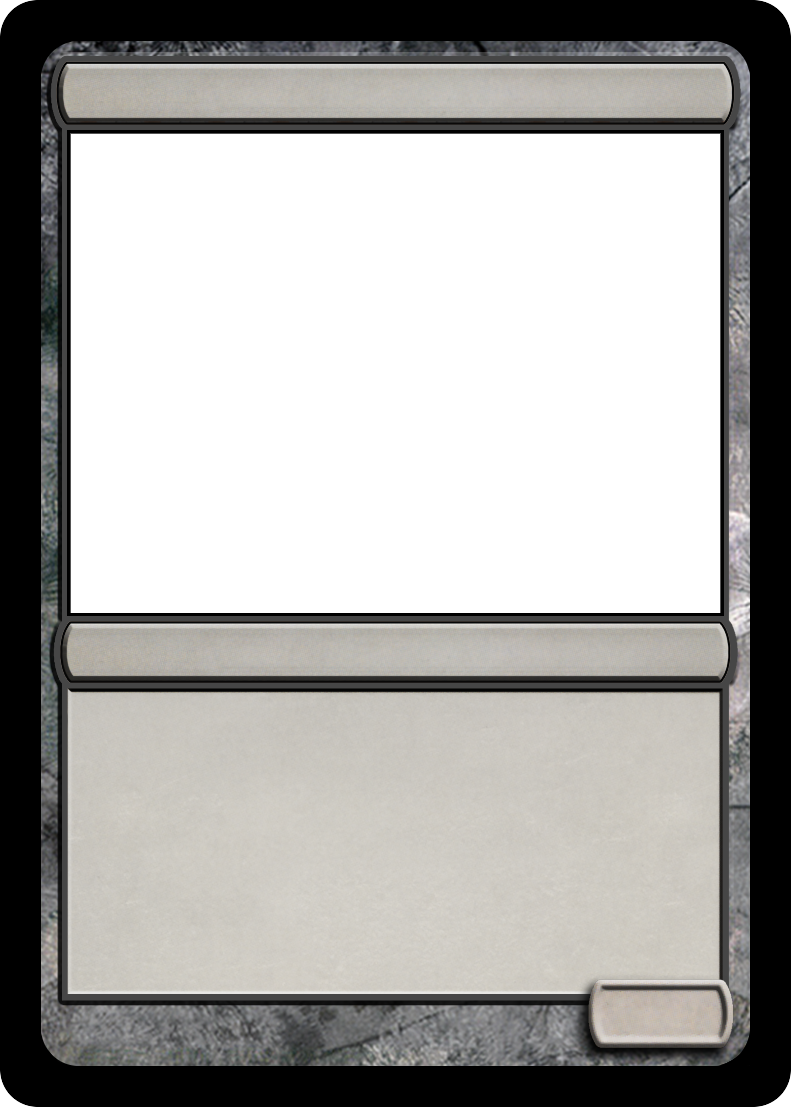
\includegraphics[width=\cardwidth cm, height=\cardheight cm]{fonds/fond_neutre.png}};

    %Titre
	\node[anchor=center] at (\titleX,\titleY) {\titlefont ENS};

	%Image
	\node[anchor=center] at (\imageX,\imageY) {
\includegraphics[width=\imageWidth px, height=\imageHeight px]{images/levreth.jpg}};
	\node[anchor=center] at (6.1,4.5) {
\includegraphics[width=12 px, height=6 px]{fonds2/legacy.jpg}};

	%Type
	\node[anchor=center] at (\typeX,\typeY) {\typefont Neutre};

	%Description
	\node[anchor=north west, text width=5.6cm] (description) at (\descriptionX,\descriptionY) {\descriptionfont\setsize{7} Vous brainstormez sur quel nom de domaine acheter. Chaque joueur doit donner un mot se terminant par le son 'ette' après vous, chacun son tour. Le premier qui hésite plus de 3 secondes pioche une carte. \par};

	%Punchline
	\node[anchor=north west, text width=5.6cm, below = 1pt of description] (punchline) {\punchlinefont\setsize{7}``Il est toujour dispo Levr.eth ? Si seulement quelqu'un avait poussé ENS en interne \ldots''\par};

	%Separateur !!!!!PAS TOUCHE!!!!!
	\fill[black,path fading=west] (description.south west) rectangle (punchline.north);
	\fill[black,path fading=east] (punchline.north) rectangle (description.south east);

	%Numéro !!!!!PAS TOUCHE!!!!!
	\node[anchor=center] at (\numberX,\numberY) {\numberfont \cardnumber};
\end{tikzpicture}\verso %Verso

%!TEX root = lot1.tex

%%%%%%%%%%%%%%%%%%%%%%%%%%%%%%%%%%%%%%%%%%%%%%%%%%%%%%%%%%%%%%%%% WEEKLY
\begin{tikzpicture} %Recto
	%Fond
    \node[anchor=south west,inner sep=0] (carte) at (0,0) {
\includegraphics[width=7.1 cm, height=9.6 cm]{fonds/noir.png}};
    \node[anchor=center] at (carte.center) {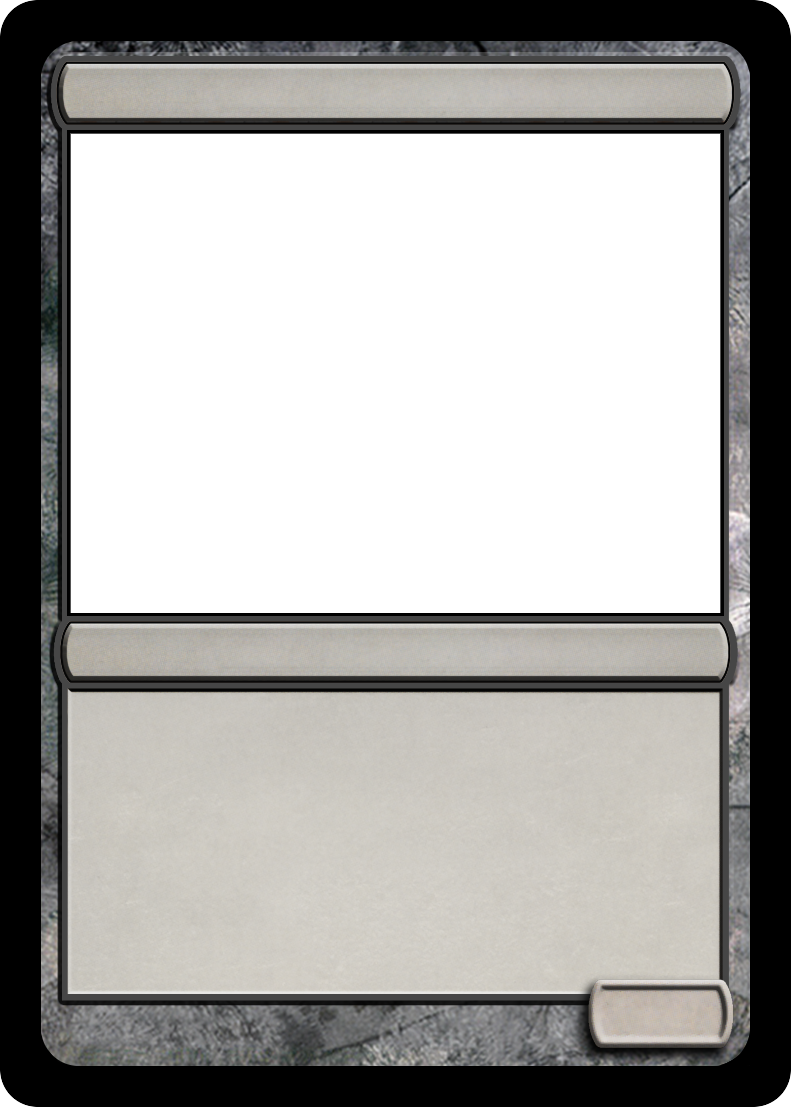
\includegraphics[width=\cardwidth cm, height=\cardheight cm]{fonds/fond_neutre.png}};

    %Titre
	\node[anchor=center] at (\titleX,\titleY) {\titlefont Monday Weekly};

	%Image
	\node[anchor=center] at (\imageX,\imageY) {
\includegraphics[width=\imageWidth px, height=\imageHeight px]{images/weekly.jpg}};
	\node[anchor=center] at (6.1,4.5) {
\includegraphics[width=12 px, height=6 px]{fonds2/legacy.jpg}};

	%Type
	\node[anchor=center] at (\typeX,\typeY) {\typefont Neutre};

	%Description
	\node[anchor=north west, text width=5.6cm] (description) at (\descriptionX,\descriptionY) {\descriptionfont\setsize{8}Chaque joueur doit nommer une carte que le joueur à sa gauche (néant si neutralisé) a joué le tour dernier. En cas d’erreur il pioche, si correct il défausse. Faites semblant d’écouter les autres joueurs comme tout le monde.\par};
	%Punchline
	\node[anchor=north west, text width=5.6cm, below = 1pt of description] (punchline) {\punchlinefont\setsize{8}``Petit tour de table, allô, Thomas tu nous entend ?''\par};

	%Separateur !!!!!PAS TOUCHE!!!!!
	\fill[black,path fading=west] (description.south west) rectangle (punchline.north);
	\fill[black,path fading=east] (punchline.north) rectangle (description.south east);

	%Numéro !!!!!PAS TOUCHE!!!!!
	\node[anchor=center] at (\numberX,\numberY) {\numberfont \cardnumber};
\end{tikzpicture}\verso %Verso
%--------------------------CARTES MALUS-------------------------------------------------------------------------------------------------

\begin{tikzpicture} %Recto
	%Fond
    \node[anchor=south west,inner sep=0] (carte) at (0,0) {
\includegraphics[width=7.1 cm, height=9.6 cm]{fonds/noir.png}};
    \node[anchor=center] at (carte.center) {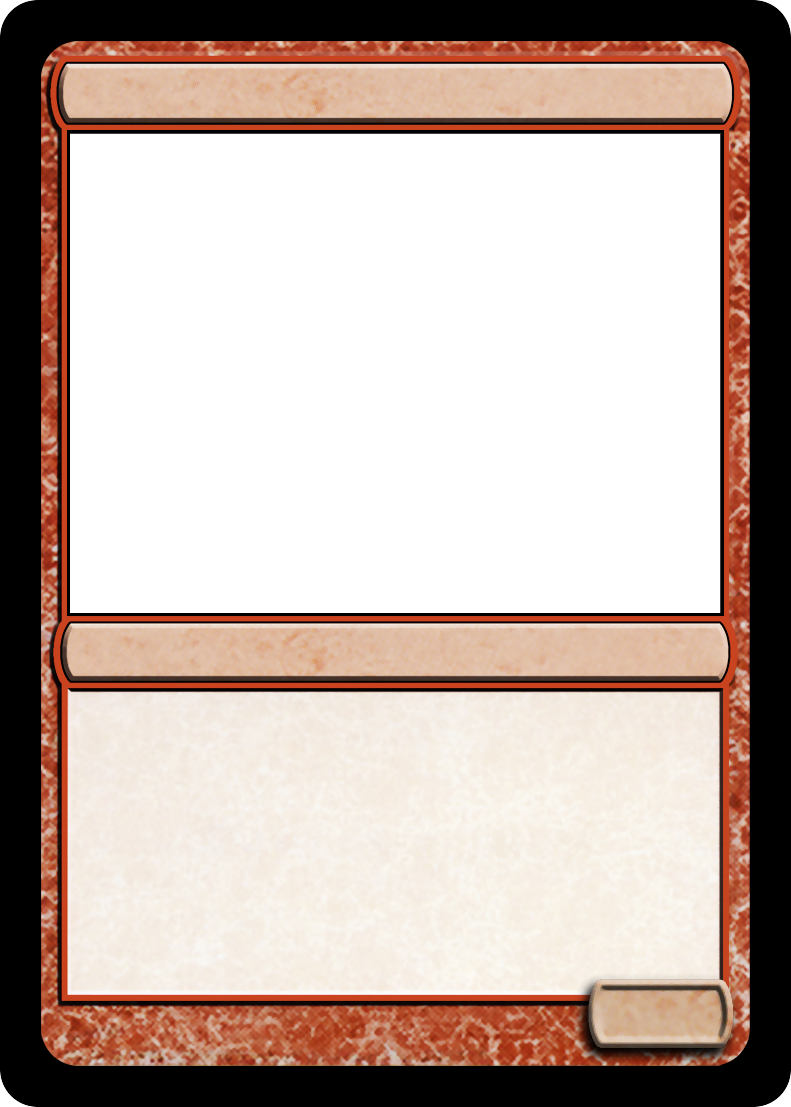
\includegraphics[width=\cardwidth cm, height=\cardheight cm]{fonds/fond_malus.png}};

    %Titre
	\node[anchor=center] at (\titleX,\titleY) {\titlefont Déplacement à Vierzon};

	%Image
	\node[anchor=center] at (\imageX,\imageY) {
\includegraphics[width=\imageWidth px, height=\imageHeight px]{images/vierzon.jpg}};
	\node[anchor=center] at (6.1,4.5) {
\includegraphics[width=12 px, height=6 px]{fonds2/legacy.jpg}};

	%Type
	\node[anchor=center] at (\typeX,\typeY) {\typefont Malus };

	%Description
	\node[anchor=north west, text width=5.6cm] (description) at (\descriptionX,\descriptionY) {\descriptionfont\setsize{8}Le joueur de votre choix part en mission à Vierzon la paradisiaque pour configurer un HSM foireux et pioche immédiatement une carte.\par};
	%Punchline
	\node[anchor=north west, text width=5.6cm, below = 1pt of description] (punchline) {\punchlinefont\setsize{8}``Vous espérez que vos vaccins sont bien à jour.''\par};

	%Separateur !!!!!PAS TOUCHE!!!!!
	\fill[black,path fading=west] (description.south west) rectangle (punchline.north);
	\fill[black,path fading=east] (punchline.north) rectangle (description.south east);

	%Numéro !!!!!PAS TOUCHE!!!!!
	\node[anchor=center] at (\numberX,\numberY) {\numberfont \cardnumber};
\end{tikzpicture}\verso %Verso


\begin{tikzpicture} %Recto
	%Fond
    \node[anchor=south west,inner sep=0] (carte) at (0,0) {
\includegraphics[width=7.1 cm, height=9.6 cm]{fonds/noir.png}};
    \node[anchor=center] at (carte.center) {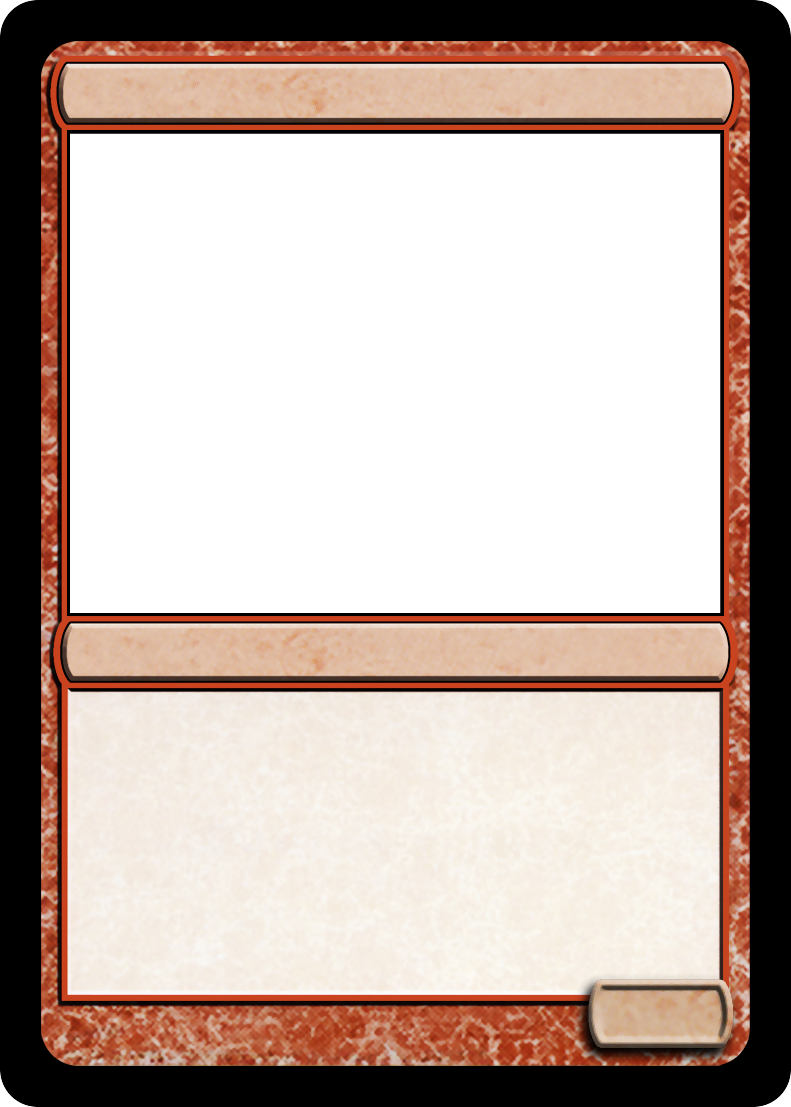
\includegraphics[width=\cardwidth cm, height=\cardheight cm]{fonds/fond_malus.png}};

    %Titre
	\node[anchor=center] at (\titleX,\titleY) {\titlefont Pizza Faille-V};

	%Image
	\node[anchor=center] at (\imageX,\imageY) {
\includegraphics[width=\imageWidth px, height=\imageHeight px]{images/pizza5.jpg}};
	\node[anchor=center] at (6.1,4.5) {
\includegraphics[width=12 px, height=6 px]{fonds2/legacy.jpg}};

	%Type
	\node[anchor=center] at (\typeX,\typeY) {\typefont Malus };

	%Description
	\node[anchor=north west, text width=5.6cm] (description) at (\descriptionX,\descriptionY) {\descriptionfont\setsize{8} Lorsque vous jouez cette carte, chaque joueur ayant exactement 5 cartes en main fait une intoxication alimentaire suite à la distribution généreuse de pizzas Faille-V à la fraicheur douteuse.\par};
	%Punchline
	\node[anchor=north west, text width=5.6cm, below = 1pt of description] (punchline) {\punchlinefont\setsize{8}``Budget is low man.''\par};

	%Separateur !!!!!PAS TOUCHE!!!!!
	\fill[black,path fading=west] (description.south west) rectangle (punchline.north);
	\fill[black,path fading=east] (punchline.north) rectangle (description.south east);

	%Numéro !!!!!PAS TOUCHE!!!!!
	\node[anchor=center] at (\numberX,\numberY) {\numberfont \cardnumber};
\end{tikzpicture}\verso %Verso


%%%%%%%%%%%%%%%%%%%%%%%%%%%%%%%%% ELEVO
\begin{tikzpicture} %Recto
	%Fond
    \node[anchor=south west,inner sep=0] (carte) at (0,0) {
\includegraphics[width=7.1 cm, height=9.6 cm]{fonds/noir.png}};
    \node[anchor=center] at (carte.center) {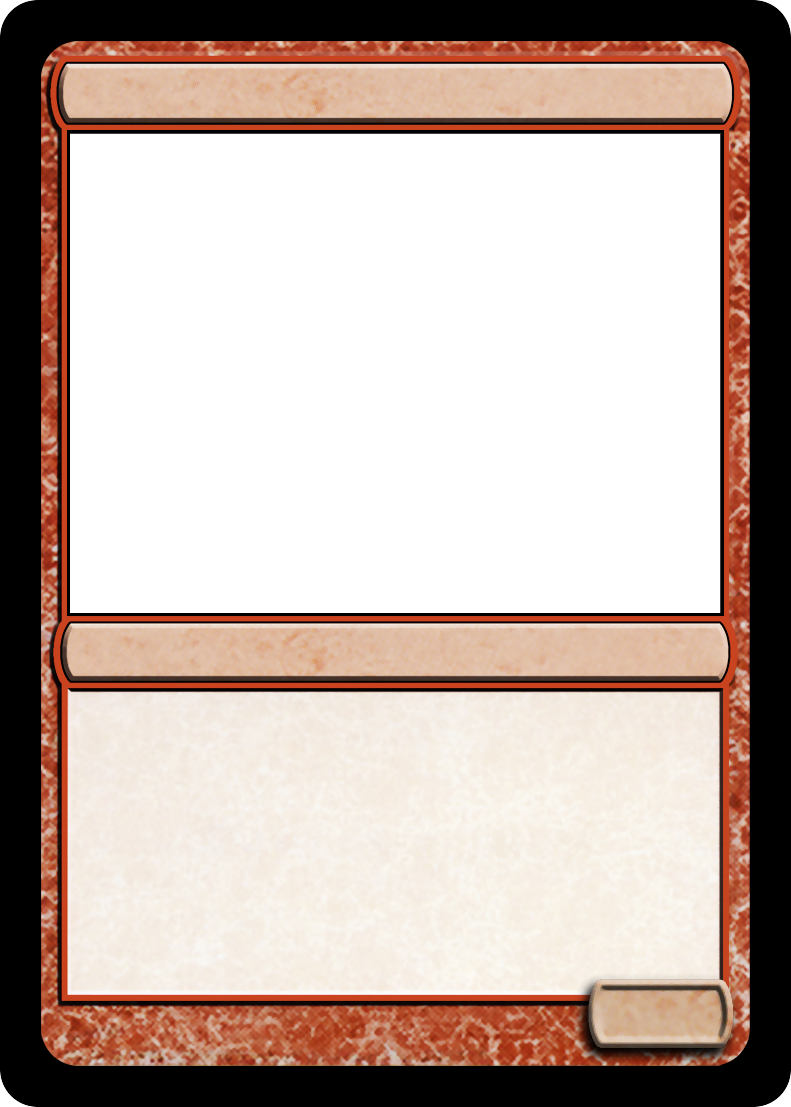
\includegraphics[width=\cardwidth cm, height=\cardheight cm]{fonds/fond_malus.png}};

    %Titre
	\node[anchor=center] at (\titleX,\titleY) {\titlefont Hey, le Veau !};

	%Image
	\node[anchor=center] at (\imageX,\imageY) {
\includegraphics[width=\imageWidth px, height=\imageHeight px]{images/veau.jpg}};
	\node[anchor=center] at (6.1,4.5) {
\includegraphics[width=12 px, height=6 px]{fonds2/legacy.jpg}};

	%Type
	\node[anchor=center] at (\typeX,\typeY) {\typefont Malus };

	%Description
	\node[anchor=north west, text width=5.6cm] (description) at (\descriptionX,\descriptionY) {\descriptionfont\setsize{6} 
C'est la période des évaluations, l'autre joueur de votre choix doit se mettre à genou devant le manager. 
Ces derniers font une bataille avec deux cartes de leur choix, révèle la valeur, le gagnant défausse une carte, 
 le perdant en pioche une.\par};
	%Punchline
	\node[anchor=north west, text width=5.6cm, below = 1pt of description] (punchline) {\punchlinefont\setsize{6}``Exode 32: Ils se sont fabriqué un veauu [...] se sont mis à genoux devant lui, 
et ils lui ont offert des sacrifices.''\par};

	%Separateur !!!!!PAS TOUCHE!!!!!
	\fill[black,path fading=west] (description.south west) rectangle (punchline.north);
	\fill[black,path fading=east] (punchline.north) rectangle (description.south east);

	%Numéro !!!!!PAS TOUCHE!!!!!
	\node[anchor=center] at (\numberX,\numberY) {\numberfont \cardnumber};
\end{tikzpicture}\verso %Verso


%%%%%%%%%%%%%%%%%%%%%%%%%%%%%%%%% SHITCOIN
\begin{tikzpicture} %Recto
	%Fond
    \node[anchor=south west,inner sep=0] (carte) at (0,0) {
\includegraphics[width=7.1 cm, height=9.6 cm]{fonds/noir.png}};
    \node[anchor=center] at (carte.center) {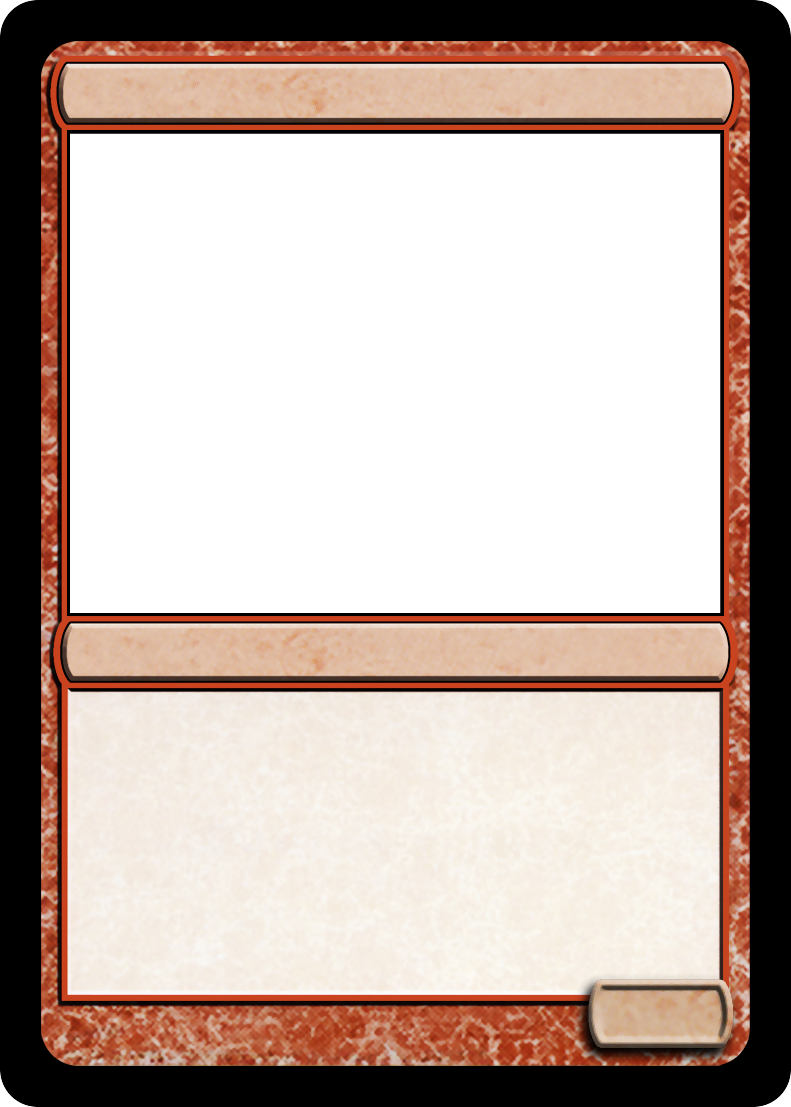
\includegraphics[width=\cardwidth cm, height=\cardheight cm]{fonds/fond_malus.png}};

    %Titre
	\node[anchor=center] at (\titleX,\titleY) {\titlefont Shitcoin en baisse};

	%Image
	\node[anchor=center] at (\imageX,\imageY) {
\includegraphics[width=\imageWidth px, height=\imageHeight px]{images/shitcoin.jpg}};
	\node[anchor=center] at (6.1,4.5) {
\includegraphics[width=12 px, height=6 px]{fonds2/legacy.jpg}};

	%Type
	\node[anchor=center] at (\typeX,\typeY) {\typefont Malus };

	%Description
	\node[anchor=north west, text width=5.6cm] (description) at (\descriptionX,\descriptionY) {\descriptionfont\setsize{6} 
Oh non ! Le joueur ciblé a trop écouté les conseils d'Adrien et placé des tokens dans un shitcoin qui vient de dégringoler ! Il place l'un des tokens de son Nano dans la défausse\par};
	%Punchline
	\node[anchor=north west, text width=5.6cm, below = 1pt of description] (punchline) {\punchlinefont\setsize{6}``Don't worry for him, Adrien avait vendu les siens.''\par};

	%Separateur !!!!!PAS TOUCHE!!!!!
	\fill[black,path fading=west] (description.south west) rectangle (punchline.north);
	\fill[black,path fading=east] (punchline.north) rectangle (description.south east);

	%Numéro !!!!!PAS TOUCHE!!!!!
	\node[anchor=center] at (\numberX,\numberY) {\numberfont \cardnumber};
\end{tikzpicture}\verso %Verso




%%%%%%%%%%%%%%%%%%%%%%%%%%%%%%%%% ANANAS
\begin{tikzpicture} %Recto
	%Fond
    \node[anchor=south west,inner sep=0] (carte) at (0,0) {
\includegraphics[width=7.1 cm, height=9.6 cm]{fonds/noir.png}};
    \node[anchor=center] at (carte.center) {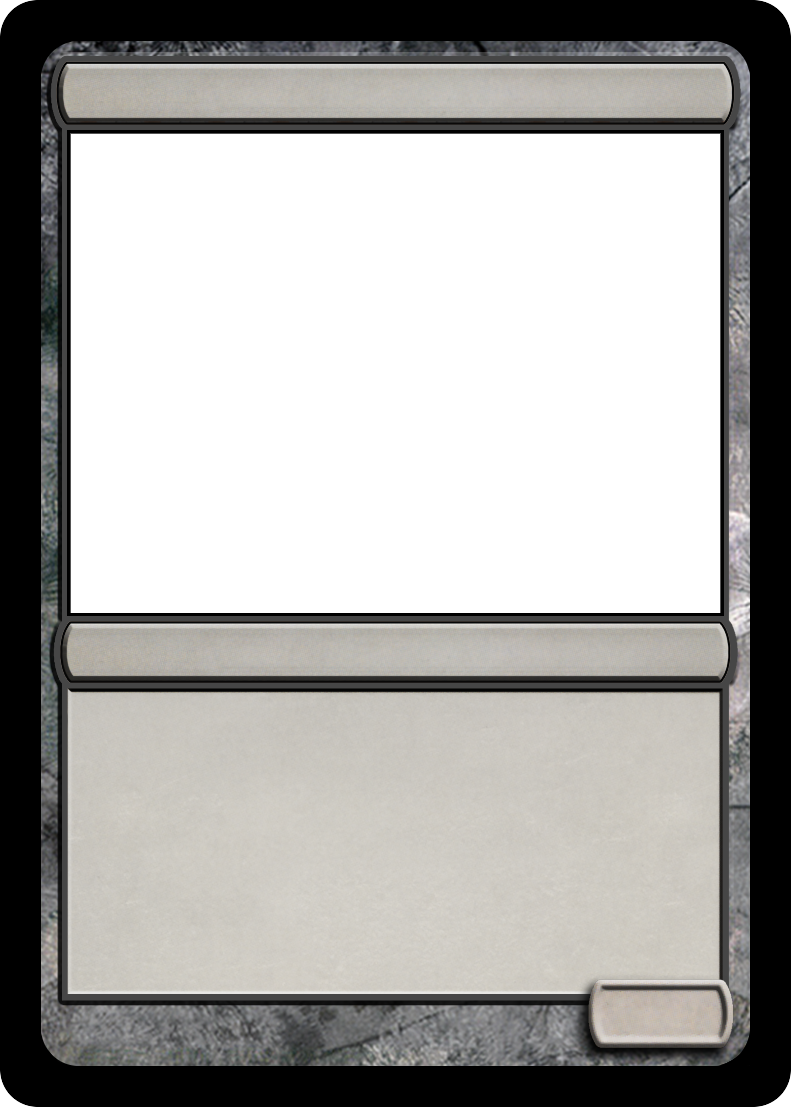
\includegraphics[width=\cardwidth cm, height=\cardheight cm]{fonds/fond_neutre.png}};

    %Titre
	\node[anchor=center] at (\titleX,\titleY) {\titlefont Hot Ananas !};

	%Image
	\node[anchor=center] at (\imageX,\imageY) {
\includegraphics[width=\imageWidth px, height=\imageHeight px]{images/ananas.jpg}};
	\node[anchor=center] at (6.1,4.5) {
\includegraphics[width=12 px, height=6 px]{fonds2/legacy.jpg}};

	%Type
	\node[anchor=center] at (\typeX,\typeY) {\typefont Neutre };

	%Description
	\node[anchor=north west, text width=5.6cm] (description) at (\descriptionX,\descriptionY) {\descriptionfont\setsize{6} 
N'écoutant que votre bon coeur, et malgré les polémiques autour de ce fruit controversé, vous décidez de contribuer au Pineapple Fund. Prenez un token de votre Nano et mettez le dans la défausse.\par};
	%Punchline
	\node[anchor=north west, text width=5.6cm, below = 1pt of description] (punchline) {\punchlinefont\setsize{6}``Cet ananas est très chaud !''\par};

	%Separateur !!!!!PAS TOUCHE!!!!!
	\fill[black,path fading=west] (description.south west) rectangle (punchline.north);
	\fill[black,path fading=east] (punchline.north) rectangle (description.south east);

	%Numéro !!!!!PAS TOUCHE!!!!!
	\node[anchor=center] at (\numberX,\numberY) {\numberfont \cardnumber};
\end{tikzpicture}\verso %Verso



%%%%%%%%%%%%%%%%%%%%%%%%%%%%%%%%% KICKASS
\begin{tikzpicture} %Recto
	%Fond
    \node[anchor=south west,inner sep=0] (carte) at (0,0) {
\includegraphics[width=7.1 cm, height=9.6 cm]{fonds/noir.png}};
    \node[anchor=center] at (carte.center) {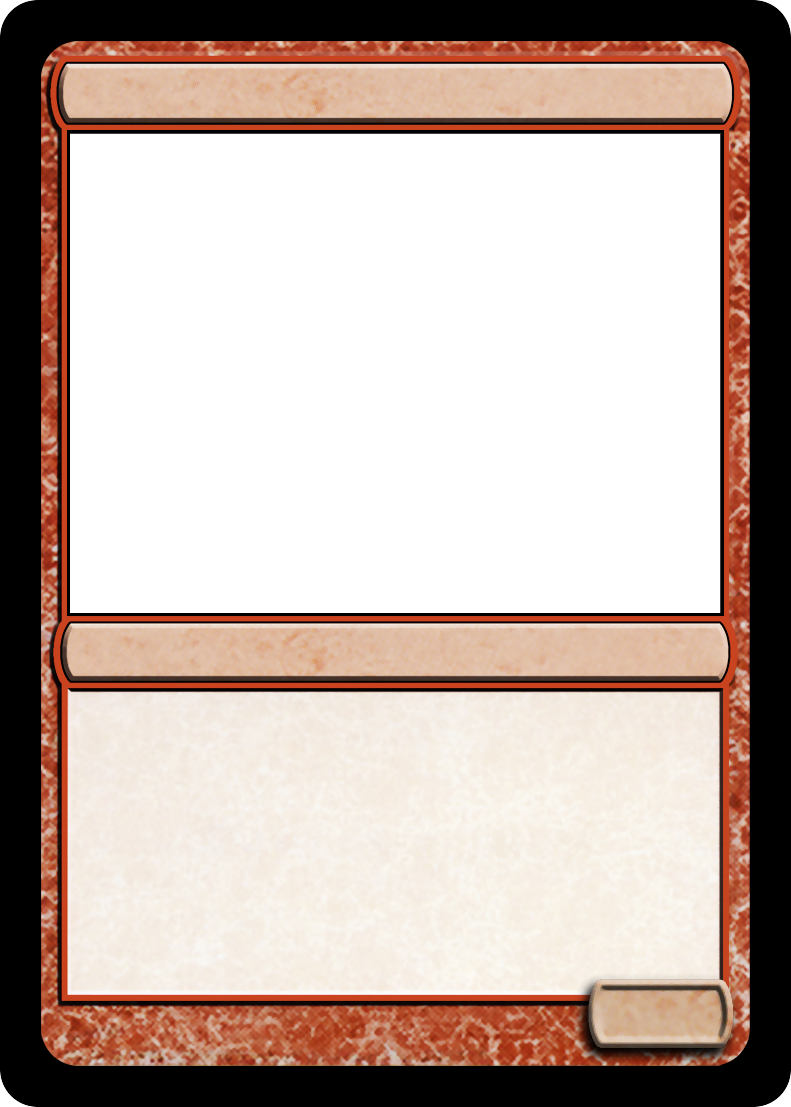
\includegraphics[width=\cardwidth cm, height=\cardheight cm]{fonds/fond_malus.png}};

    %Titre
	\node[anchor=center] at (\titleX,\titleY) {\titlefont PM éconduit};

	%Image
	\node[anchor=center] at (\imageX,\imageY) {\includegraphics[width=\imageWidth px, height=\imageHeight px]{images/kickass.jpg}};
	\node[anchor=center] at (6.1,4.5) {\includegraphics[width=12 px, height=6 px]{fonds2/legacy.jpg}};

	%Type
	\node[anchor=center] at (\typeX,\typeY) {\typefont Malus};

	%Description
	\node[anchor=north west, text width=5.6cm] (description) at (\descriptionX,\descriptionY) {\descriptionfont\setsize{6} 
Par les hasards d'une gestion fine et maîtrisé, le contrat du PM n'est pas reconduit. Le joueur PM à ce tour doit piocher une carte. La carte du PM est mise de côté et ne pourra pas être choisie au tour prochain.\par};
	%Punchline
	\node[anchor=north west, text width=5.6cm, below = 1pt of description] (punchline) {\punchlinefont\setsize{6}``Il a été dégagé comme un clochard holder de XRP atteint de Monkey Pox !''\par};

	%Separateur !!!!!PAS TOUCHE!!!!!
	\fill[black,path fading=west] (description.south west) rectangle (punchline.north);
	\fill[black,path fading=east] (punchline.north) rectangle (description.south east);

	%Numéro !!!!!PAS TOUCHE!!!!!
	\node[anchor=center] at (\numberX,\numberY) {\numberfont \cardnumber};
\end{tikzpicture}\verso %Verso



%%%%%%%%%%%%%%%%%%%%%%%%%%%%%%%%% VOL DE PR
\begin{tikzpicture} %Recto
	%Fond
    \node[anchor=south west,inner sep=0] (carte) at (0,0) {\includegraphics[width=7.1 cm, height=9.6 cm]{fonds/noir.png}};
    \node[anchor=center] at (carte.center) {\includegraphics[width=\cardwidth cm, height=\cardheight cm]{fonds/fond_malus.png}};

    %Titre
	\node[anchor=center] at (\titleX,\titleY) {\titlefont Vol de PR};

	%Image
	\node[anchor=center] at (\imageX,\imageY) {\includegraphics[width=\imageWidth px, height=\imageHeight px]{images/thief.jpg}};
	\node[anchor=center] at (6.1,4.5) {\includegraphics[width=12 px, height=6 px]{fonds2/legacy.jpg}};

	%Type
	\node[anchor=center] at (\typeX,\typeY) {\typefont Malus};

	%Description
	\node[anchor=north west, text width=5.6cm] (description) at (\descriptionX,\descriptionY) {\descriptionfont\setsize{6} 
Pourquoi coder une PR quand on peut simplement mettre son nom sur celle d'un autre ? Vous pouvez jouer cette carte pendant le tour d'un autre joueur pour récupérer le fruit de ses efforts (la dernière carte tokenisée dans son Nano, vers le votre).\par};
	%Punchline
	\node[anchor=north west, text width=5.6cm, below = 1pt of description] (punchline) {\punchlinefont\setsize{6}``Je suis deg', je me suis fait Thomas !''\par};

	%Separateur !!!!!PAS TOUCHE!!!!!
	\fill[black,path fading=west] (description.south west) rectangle (punchline.north);
	\fill[black,path fading=east] (punchline.north) rectangle (description.south east);

	%Numéro !!!!!PAS TOUCHE!!!!!
	\node[anchor=center] at (\numberX,\numberY) {\numberfont \cardnumber};
\end{tikzpicture}\verso %Verso




%%%%%%%%%%%%%%%%%%%%%%%%%%%%%%%%% LOOK IT UP !
\begin{tikzpicture} %Recto
	%Fond
    \node[anchor=south west,inner sep=0] (carte) at (0,0) {\includegraphics[width=7.1 cm, height=9.6 cm]{fonds/noir.png}};
    \node[anchor=center] at (carte.center) {\includegraphics[width=\cardwidth cm, height=\cardheight cm]{fonds/fond_neutre.png}};

    %Titre
	\node[anchor=center] at (\titleX,\titleY) {\titlefont Look it Up !};

	%Image
	\node[anchor=center] at (\imageX,\imageY) {\includegraphics[width=\imageWidth px, height=\imageHeight px]{images/camel.jpg}};
	\node[anchor=center] at (6.1,4.5) {\includegraphics[width=12 px, height=6 px]{fonds2/legacy.jpg}};

	%Type
	\node[anchor=center] at (\typeX,\typeY) {\typefont Neutre};

	%Description
	\node[anchor=north west, text width=5.6cm] (description) at (\descriptionX,\descriptionY) {\descriptionfont\setsize{6} 
Le Chameau vous intime de regarder en haut. Le joueur ciblé passe le reste de son tour à regarder le plafond et apprendre son métier du joueur le moins compétent (celui qui a le plus de cartes en main) jusqu'à la fin du tour. Il pioche une carte pour le temps inutilement perdu à le convaincre de l'inutilité de la démarche.\par};
	%Punchline
	\node[anchor=north west, text width=5.6cm, below = 1pt of description] (punchline) {\punchlinefont\setsize{6}``Bon entre le chameau et Di Caprio, qui écouter ? Look Up or not ?''\par};

	%Separateur !!!!!PAS TOUCHE!!!!!
	\fill[black,path fading=west] (description.south west) rectangle (punchline.north);
	\fill[black,path fading=east] (punchline.north) rectangle (description.south east);

	%Numéro !!!!!PAS TOUCHE!!!!!
	\node[anchor=center] at (\numberX,\numberY) {\numberfont \cardnumber};
\end{tikzpicture}\verso %Verso




%%%%%%%%%%%%%%%%%%%%%%%%%%%%%%%%% GROS TAS !
\begin{tikzpicture} %Recto
	%Fond
    \node[anchor=south west,inner sep=0] (carte) at (0,0) {\includegraphics[width=7.1 cm, height=9.6 cm]{fonds/noir.png}};
    \node[anchor=center] at (carte.center) {\includegraphics[width=\cardwidth cm, height=\cardheight cm]{fonds/fond_neutre.png}};

    %Titre
	\node[anchor=center] at (\titleX,\titleY) {\titlefont Gros Tas};

	%Image
	\node[anchor=center] at (\imageX,\imageY) {\includegraphics[width=\imageWidth px, height=\imageHeight px]{images/grostas.jpg}};
	\node[anchor=center] at (6.1,4.5) {\includegraphics[width=12 px, height=6 px]{fonds2/legacy.jpg}};

	%Type
	\node[anchor=center] at (\typeX,\typeY) {\typefont Neutre};

	%Description
	\node[anchor=north west, text width=5.6cm] (description) at (\descriptionX,\descriptionY) {\descriptionfont\setsize{6} 
	Trop de passage au AKI vous ont fait prendre beaucoup de poids, allez donc vous exercer un peu. Le joueur ciblé fait des pompes jusqu'à la fin du tour et réfléchit au prochain prototype Ledger.\par};
	%Punchline
	\node[anchor=north west, text width=5.6cm, below = 1pt of description] (punchline) {\punchlinefont\setsize{6}``En espérant qu'il ne finisse pas dans un train sans retour comme 	GrosQuick''\par};

	%Separateur !!!!!PAS TOUCHE!!!!!
	\fill[black,path fading=west] (description.south west) rectangle (punchline.north);
	\fill[black,path fading=east] (punchline.north) rectangle (description.south east);

	%Numéro !!!!!PAS TOUCHE!!!!!
	\node[anchor=center] at (\numberX,\numberY) {\numberfont \cardnumber};
\end{tikzpicture}\verso %Verso





